\section{Results and Discussion}
\label{sec:Results_and_Discussion}
This section contains lists of all important results and summarizes the most important things.

\subsection{Comparability}
\label{subsec:Comparability}
To be able to compare the fitted results agains a calculated value, equation \ref{eq:cylindrical_coil_b0} is used to compute the vacuum permeability $\mu_0$. In order to obtain the desired result, the formula must be rearranged like this:
\begin{equation}
\mu_0=\frac{B_0l}{NI}\cdot\sqrt{1+(\,^{2R}\!/_{l})^2}
\label{eq:cylindrical_coil_mu_0}
\end{equation}

\subsection{Results Short Coil (Central Value)}
\label{subsec:Results_Short_Coil_Central}
The calculated value has been computed with equation \ref{eq:cylindrical_coil_mu_0}.
\begin{table}[H]
	\centering
	\renewcommand{\arraystretch}{1.3}
	\begin{tabular}{r l}
		\hline
		\textbf{Calculated} $\mu_0$ & $(1.25235\pm0.01922)\cdot10^{-6}\ \,^\text{Vs}\!/_\text{Am}$ \\
		\textbf{Fitted} $\mu_0$ & $(1.25396\pm0.00019)\cdot10^{-6}\ \,^\text{Vs}\!/_\text{Am}$ \\ \hline
	\end{tabular}
	\caption{Results Short Coil (Central Value)}
	\label{tab:Results_Short_Coil_Central}
\end{table}
The calculated and fitted values are pretty close to each other. The big difference is the uncertainty which is way bigger for the calculated value. This is plausible because it contains not only statistical but also systematic uncertainty. This is shown in the following figure \ref{fig:Graphical_Comparison_Short_Center}:
\begin{figure}[H]
	\centering
	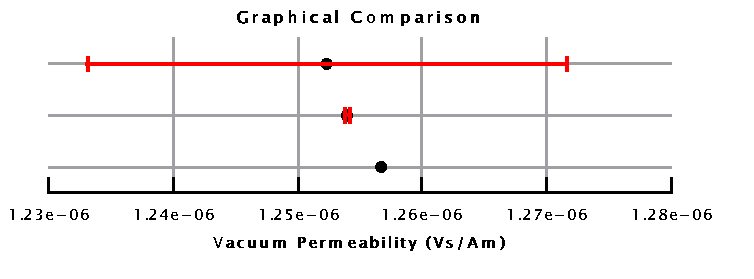
\includegraphics[scale=1]{Graphical_Comparison_Short_Center}
	\caption{Graphical Comparison Short Coil (Center Value)}
	\label{fig:Graphical_Comparison_Short_Center}
\end{figure}
This figure shows a graphical comparison between the calculated (top), the fitted (middle) and the real value (bottom) of $\mu_0$. The red line marks the uncertainty. Obviously the real value of $\mu_0$ has no uncertainty and is thus not shown. An interesting fact is, that the real value of $\mu_0$ is not in the range of the uncertainty of the fitted value. This is due to the fact, that the systematic uncertainty is not contained.
\newpage
\subsection{Results Short Coil (Field Pattern)}
\label{subsec:Results_Short_Coil_Field}
The calculated value has again been computed with equation \ref{eq:cylindrical_coil_mu_0}.
\begin{table}[H]
	\centering
	\renewcommand{\arraystretch}{1.3}
	\begin{tabular}{r l}
		\hline
		\textbf{Calculated} $\mu_0$ & $(1.25314\pm0.01924)\cdot10^{-6}\ \,^\text{Vs}\!/_\text{Am}$ \\
		\textbf{Fitted} $\mu_0$ & $(1.25017\pm0.00063)\cdot10^{-6}\ \,^\text{Vs}\!/_\text{Am}$ \\ \hline
	\end{tabular}
	\caption{Results Short Coil (Field Pattern)}
	\label{tab:Results_Short_Coil_Field}
\end{table}
This time the calculated and the fitted value are further apart (not that much tough). This is shown in the following figure \ref{fig:Graphical_Comparison_Short_Field}:
\begin{figure}[H]
	\centering
	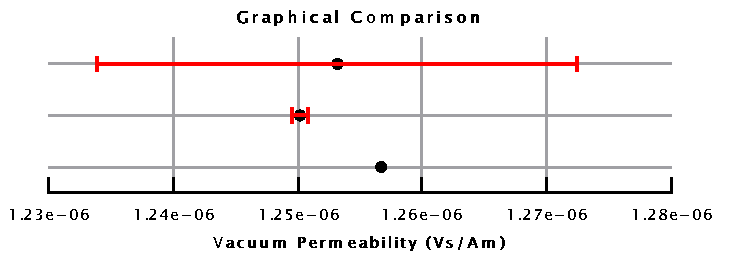
\includegraphics[scale=1]{Graphical_Comparison_Short_Field}
	\caption{Graphical Comparison Short Coil (Field Pattern)}
	\label{fig:Graphical_Comparison_Short_Field}
\end{figure}
This figure shows a graphical comparison between the calculated (top), the fitted (middle) and the real value (bottom) of $\mu_0$. The real value of $\mu_0$ is again not in the range of the uncertainty of the fitted value.

\subsection{Results Long Coil (Central Value)}
\label{subsec:Results_Long_Coil_Central}
The calculated value was once again computed with equation \ref{eq:cylindrical_coil_mu_0}.
\begin{table}[H]
	\centering
	\renewcommand{\arraystretch}{1.3}
	\begin{tabular}{r l}
		\hline
		\textbf{Calculated} $\mu_0$ & $(1.24875\pm0.01482)\cdot10^{-6}\ \,^\text{Vs}\!/_\text{Am}$ \\
		\textbf{Fitted} $\mu_0$ & $(1.24853\pm0.00016)\cdot10^{-6}\ \,^\text{Vs}\!/_\text{Am}$ \\ \hline
	\end{tabular}
	\caption{Results Long Coil (Central Value)}
	\label{tab:Results_Long_Coil_Central}
\end{table}
The calculated and the fitted values lie really close to each other. The calculated value is almost within the range of uncertainty of the fitted one. This is shown in figure \ref{fig:Graphical_Comparison_Long_Center} on the next page:
\begin{figure}[H]
	\centering
	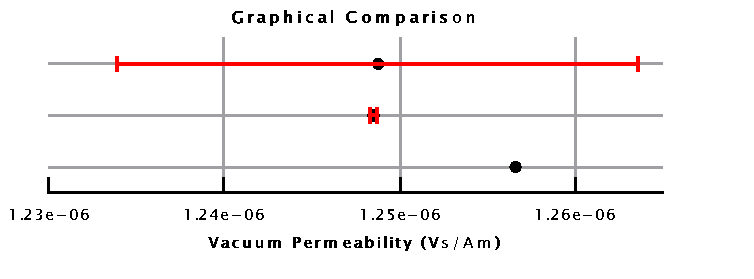
\includegraphics[scale=1]{Graphical_Comparison_Long_Center}
	\caption{Graphical Comparison Long Coil (Center Value)}
	\label{fig:Graphical_Comparison_Long_Center}
\end{figure}
This figure shows a graphical comparison between the calculated (top), the fitted (middle) and the real value (bottom) of $\mu_0$. Interesting in this figure is, that this time both the measured and the fitted value are close to each other but further apart from the real value $\mu_0$.
\subsection{Results Long Coil (Field Pattern)}
\label{subsec:Results_Long_Coil_Field}
The calculated value has as well been computed with equation \ref{eq:cylindrical_coil_mu_0}.
\begin{table}[H]
	\centering
	\renewcommand{\arraystretch}{1.3}
	\begin{tabular}{r l}
		\hline
		\textbf{Calculated} $\mu_0$ & $(1.24661\pm0.01480)\cdot10^{-6}\ \,^\text{Vs}\!/_\text{Am}$ \\
		\textbf{Fitted} $\mu_0$ & $(1.24867\pm0.00036)\cdot10^{-6}\ \,^\text{Vs}\!/_\text{Am}$ \\ \hline
	\end{tabular}
	\caption{Results Long Coil (Field Pattern)}
	\label{tab:Results_Long_Coil_Field}
\end{table}
The calculated and the fitted values are again close to each other but further apart from the true value of $\mu_0$. This is shown in the following figure \ref{fig:Graphical_Comparison_Long_Field}:
\begin{figure}[H]
	\centering
	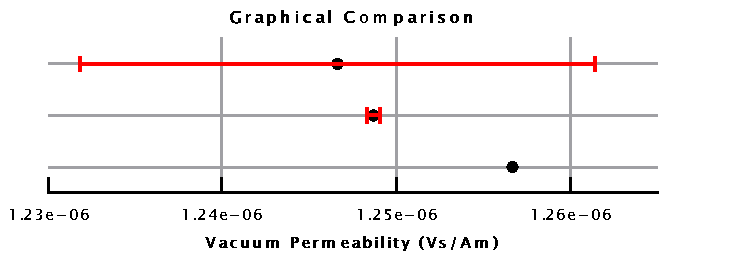
\includegraphics[scale=1]{Graphical_Comparison_Long_Field}
	\caption{Graphical Comparison Long Coil (Field Pattern)}
	\label{fig:Graphical_Comparison_Long_Field}
\end{figure}
This figure shows a graphical comparison between the calculated (top), the fitted (middle) and the real value (bottom) of $\mu_0$. Generally, the measurements with the long cylindrical coil are further apart from the real value of $\mu_0$.
